\subsection{Configuración de Backups en Bacula}

Configurar un backup en Bacula implica varios pasos críticos que aseguran que los datos importantes sean respaldados de manera eficiente y segura. A continuación, se detallan los pasos necesarios para configurar un backup dentro del sistema Bacula:

\begin{enumerate}
    \item \textbf{Definición de los Datos a Respaladar:} El primer paso en la configuración de un backup es especificar qué datos serán incluidos. Esto se realiza mediante la creación de un \textit{FileSet}, el cual incluye una lista de archivos y directorios que Bacula deberá respaldar. También se pueden especificar exclusiones dentro del mismo \textit{FileSet} para omitir archivos no necesarios o temporales.
    
    \item \textbf{Programación del Backup:} El siguiente paso es definir cuándo se realizarán los backups. Esto se configura a través de una \textit{Schedule} en Bacula, donde se pueden especificar diferentes políticas de tiempo, como backups diarios, semanales o mensuales. Cada \textit{Schedule} puede incluir múltiples eventos para manejar distintos tipos de backups (completo, incremental, diferencial) en distintos momentos.
    
    \item \textbf{Selección del Cliente:} Bacula permite realizar backups de múltiples máquinas. En este paso, se debe agregar el cliente o los clientes que serán parte del backup. Esto se define en una sección llamada \textit{Client}, donde se especifica la dirección de la máquina y otros parámetros necesarios para la comunicación y ejecución de los backups.
    
    \item \textbf{Creación del Job:} Un \textit{Job} en Bacula es la entidad que encapsula toda la información necesaria para ejecutar un backup. Incluye la vinculación del \textit{FileSet}, el \textit{Client}, y la \textit{Schedule}. Además, se debe especificar el tipo de backup y el destino del mismo, como puede ser un disco o cinta. Aquí también se definen las políticas de retención y otras opciones avanzadas.
    
    \item \textbf{Ejecución del Job:} Finalmente, una vez configurado, el job puede ser ejecutado manualmente a través de la consola de Bacula o automáticamente según la programación establecida. Durante la ejecución, Bacula gestionará la transferencia de datos desde el cliente al medio de almacenamiento especificado, siguiendo las políticas definidas en el job.
\end{enumerate}

Este proceso asegura que los datos importantes estén protegidos y que el proceso de recuperación pueda ser llevado a cabo de manera eficiente en caso de pérdida de datos o desastres.


\subsubsection{Definición de Conjuntos de Archivos (File Sets)}
Para iniciar la configuración de backups, primero definimos los conjuntos de archivos que especifican qué datos se deben respaldar. En Bacula, esto se realiza mediante la creación de File Sets, que pueden incluir diversos directorios y tipos de archivos.

\begin{figure}[H]
    \centering
    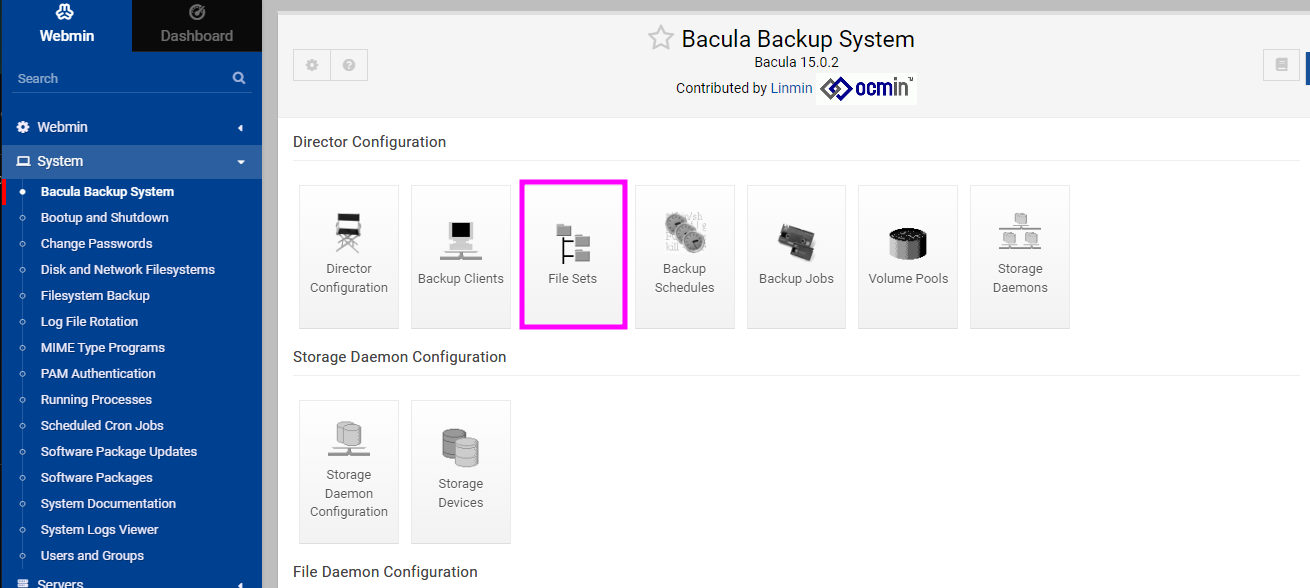
\includegraphics[width=0.5\linewidth]{instalacionBacula/filesetwebmin.png}
    \caption{Creación de un nuevo File Set en Webmin}
\end{figure}




\begin{minipage}[t]{0.45\textwidth}
    \vspace{0pt} % Alinea la parte superior de la minipágina con lo que esté al lado
    Durante la instalación, se crean algunos File Sets por defecto. Sin embargo, para fines específicos o para asegurar la integridad de datos críticos, podemos crear File Sets personalizados como se muestra a continuación:
   

    \end{minipage}%
    \hfill % Añade espacio entre las dos minipáginas si es necesario
    \begin{minipage}[t]{0.45\textwidth}
    \vspace{0pt} % Alinea la parte superior de la minipágina con lo que esté al lado
    \centering % Centra el contenido de la minipágina
      
    \begin{figure}[H]
        \centering
        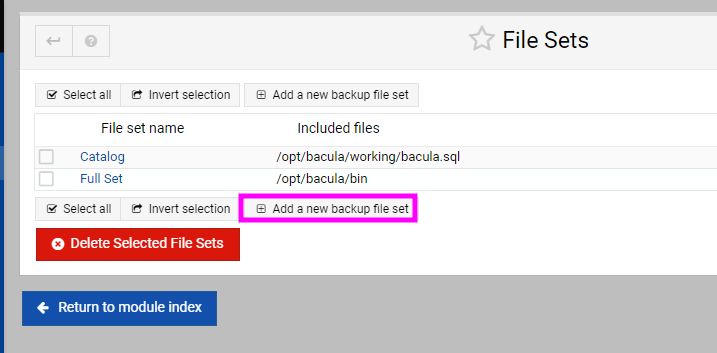
\includegraphics[width=0.95\linewidth]{instalacionBacula/cpropiofileset.png}
        \caption{Visualización de File Sets existentes}
    \end{figure}
    \end{minipage}


\smallskip






\begin{minipage}[t]{0.45\textwidth}
    \vspace{0pt} % Alinea la parte superior de la minipágina con lo que esté al lado
    En la creación de un File Set, es fundamental configurar adecuadamente las opciones disponibles, como el tipo de firma de archivo (por ejemplo, MD5 para verificación de integridad), los directorios a respaldar, y los niveles de compresión.
   

    \end{minipage}%
    \hfill % Añade espacio entre las dos minipáginas si es necesario
    \begin{minipage}[t]{0.45\textwidth}
    \vspace{0pt} % Alinea la parte superior de la minipágina con lo que esté al lado
    \centering % Centra el contenido de la minipágina
      
    
\begin{figure}[H]
    \centering
    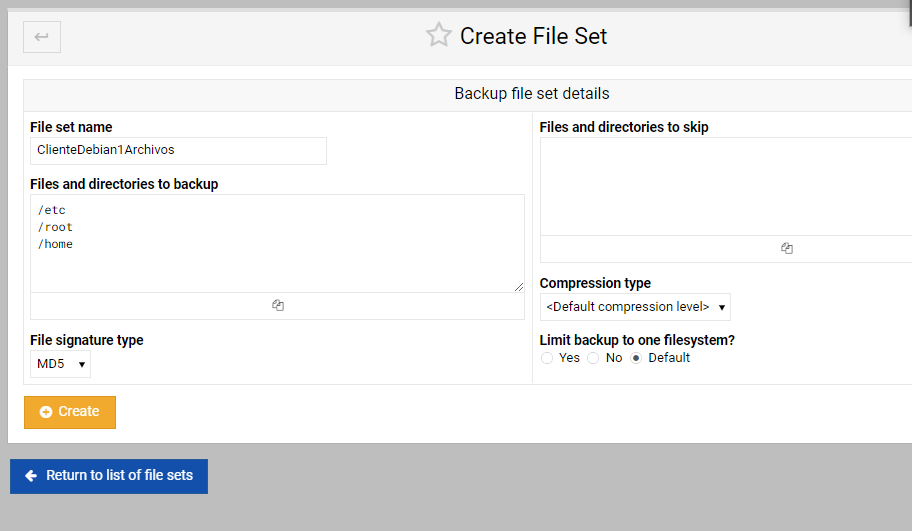
\includegraphics[width=0.95\linewidth]{instalacionBacula/createrfilesett.png}
    \caption{Configuración detallada de un File Set}
\end{figure}
    \end{minipage}


\smallskip














\subsubsection{Programación de Backups}






\begin{minipage}[t]{0.45\textwidth}
    \vspace{0pt} % Alinea la parte superior de la minipágina con lo que esté al lado
    El siguiente paso es definir cuándo se realizarán los backups, lo cual se configura mediante las programaciones de backup (schedules). Bacula permite definir múltiples programaciones para adaptarse a diferentes necesidades operativas.
   

    \end{minipage}%
    \hfill % Añade espacio entre las dos minipáginas si es necesario
    \begin{minipage}[t]{0.45\textwidth}
    \vspace{0pt} % Alinea la parte superior de la minipágina con lo que esté al lado
    \centering % Centra el contenido de la minipágina
      
    

    \begin{figure}[H]
        \centering
        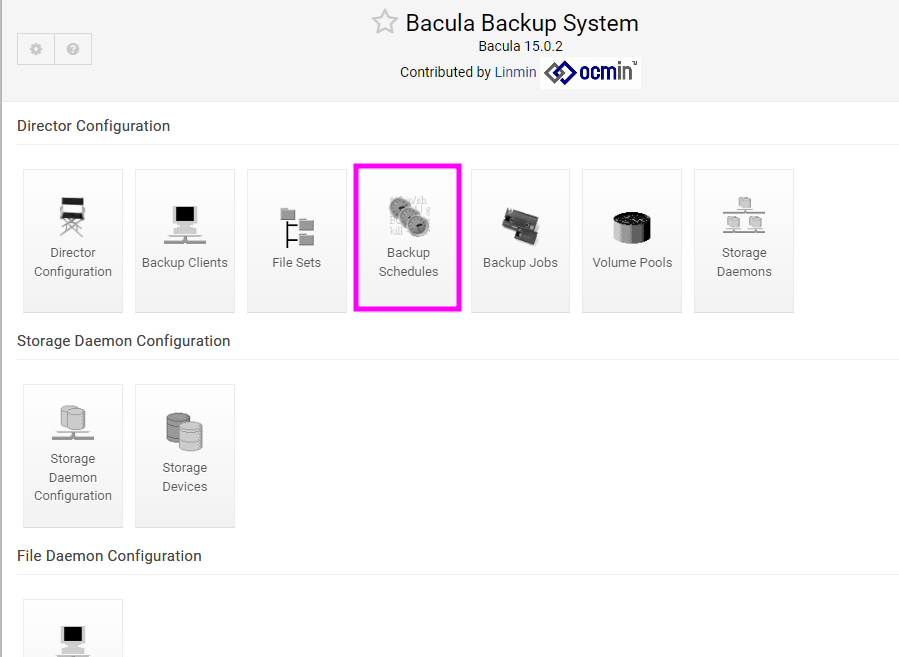
\includegraphics[width=0.95\linewidth]{instalacionBacula/schedule.png}
        \caption{Programaciones de backup existentes}
    \end{figure}
    \end{minipage}


\smallskip





Para cada necesidad específica, se puede crear una nueva programación que detalle los niveles de backup (completo, diferencial, incremental), así como la frecuencia con la que estos deben ejecutarse.

\begin{figure}[H]
    \centering
    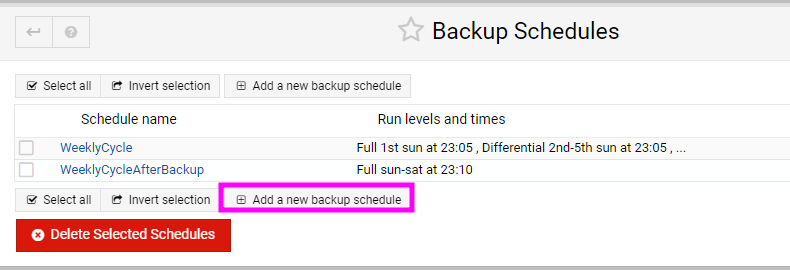
\includegraphics[width=0.5\linewidth]{instalacionBacula/newBackupSchedules.png}
    \caption{Creación de una nueva programación de backup}
\end{figure}

En la configuración de una programación, se definen los tiempos específicos y los tipos de backup, asegurando que los datos se respalden en los intervalos y formas adecuados.

\begin{figure}[H]
    \centering
    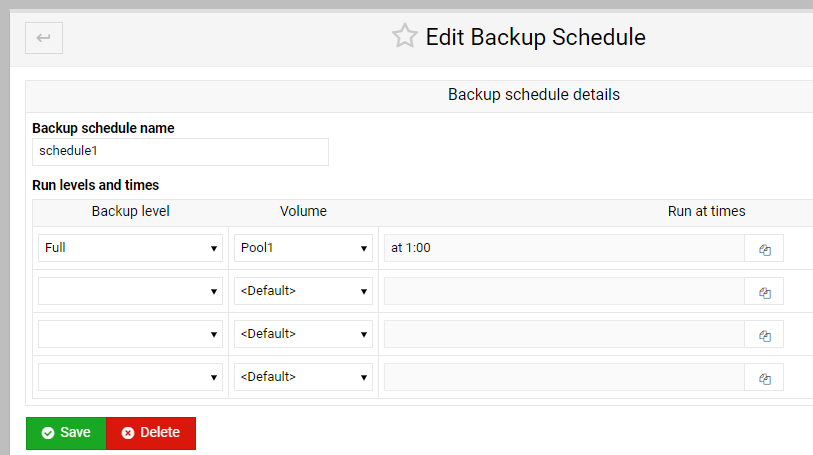
\includegraphics[width=0.5\linewidth]{instalacionBacula/editbuckupschedule.png}
    \caption{Edición de una programación de backup}
\end{figure}






\subsubsection{Clientes Respaldados}

Ahora necesitamos selecionar a quien vamos a backupear
\begin{figure}[H]
    \centering
    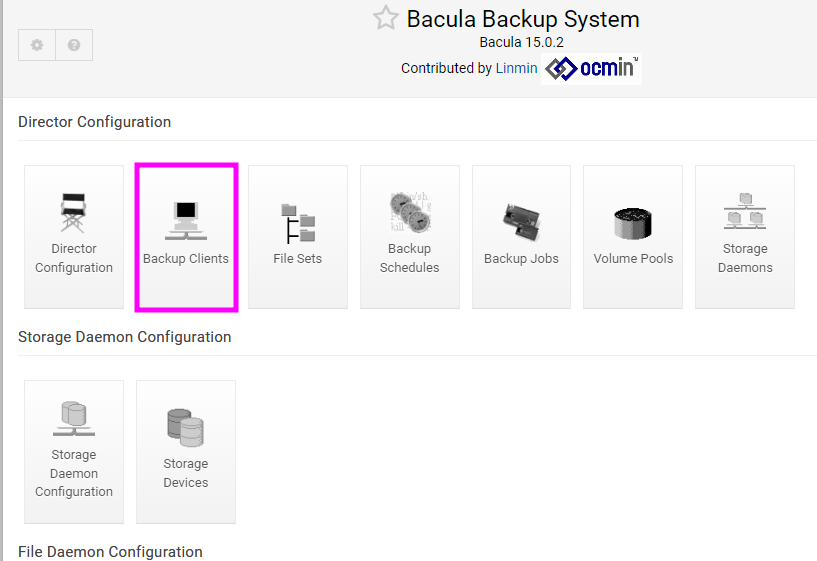
\includegraphics[width=0.5\linewidth]{instalacionBacula/asdasdas.png}
    \caption{Clientes de respaldo.}
\end{figure}

Después de definir los \textit{filesets} y los \textit{schedules}, procedemos a configurar los clientes que serán respaldados y a crear los jobs de respaldo.

\text{Añadiendo Clientes de Respaldo}

Inicialmente, el sistema tiene configurado al servidor Bacula para auto-respaldarse. Para añadir nuevos clientes:

\begin{figure}[H]
    \centering
    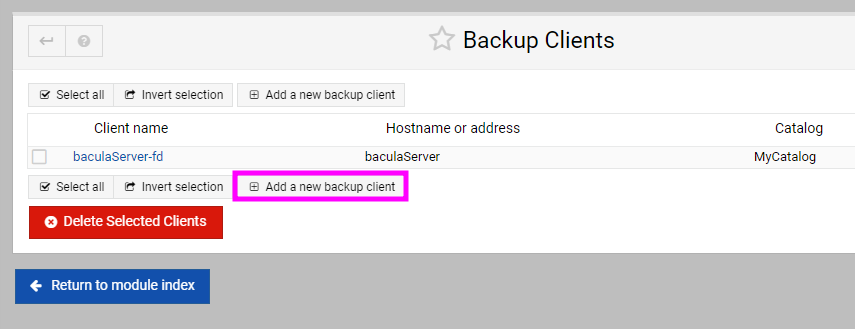
\includegraphics[width=0.5\linewidth]{instalacionBacula/addnewbuckupclient.png}
    \caption{Interfaz para añadir un nuevo cliente de respaldo.}
\end{figure}

Configuramos los detalles del nuevo cliente a respaldar:





\begin{minipage}[t]{0.45\textwidth}
    \vspace{0pt} % Alinea la parte superior de la minipágina con lo que esté al lado
    \begin{itemize}
        \item \textbf{Nombre del Cliente FD:} baculaCliente-fd
        \item \textbf{Contraseña FD de Bacula:} 
        \item \textbf{Hostname o dirección IP:} 192.168.1.116
        \item \textbf{Puerto FD de Bacula:} 9102
        \item \textbf{Catálogo a usar:} MyCatalog
        \item \textbf{Prune de trabajos y archivos caducados:} Sí
        \item \textbf{Tiempo de retención de archivos de respaldo:} 1 mes
    \end{itemize}

    \end{minipage}%
    \hfill % Añade espacio entre las dos minipáginas si es necesario
    \begin{minipage}[t]{0.45\textwidth}
    \vspace{0pt} % Alinea la parte superior de la minipágina con lo que esté al lado
    \centering % Centra el contenido de la minipágina
      
    

    
\begin{figure}[H]
    \centering
    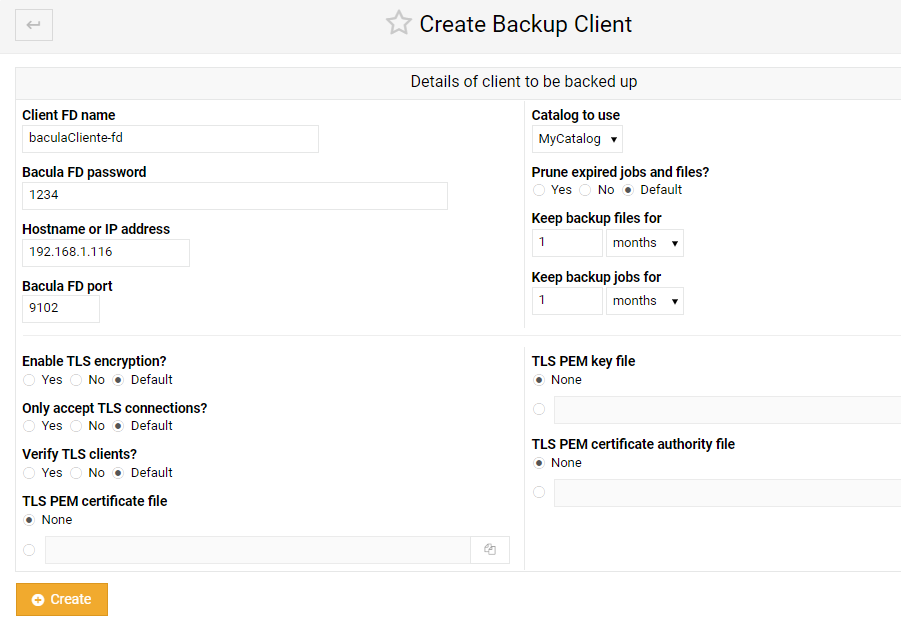
\includegraphics[width=0.95\linewidth]{instalacionBacula/detalesclienteparabuckup.png}
    \caption{Detalles del cliente a respaldar.}
\end{figure}
    \end{minipage}


\smallskip






\subsubsection{Creación y Configuración de Jobs de Respaldo}
Ahora podemos crear y ejecutar un job:

\begin{figure}[H]
    \centering
    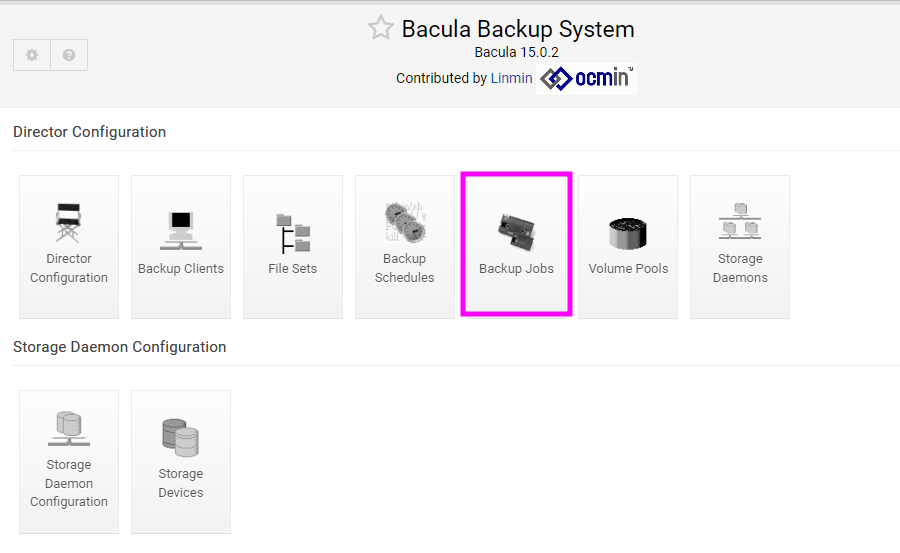
\includegraphics[width=0.5\linewidth]{instalacionBacula/createJOB.png}
    \caption{Crear un job.}
\end{figure}
Procedemos a crear un nuevo job de respaldo que utilizará las configuraciones establecidas:

\begin{figure}[H]
    \centering
    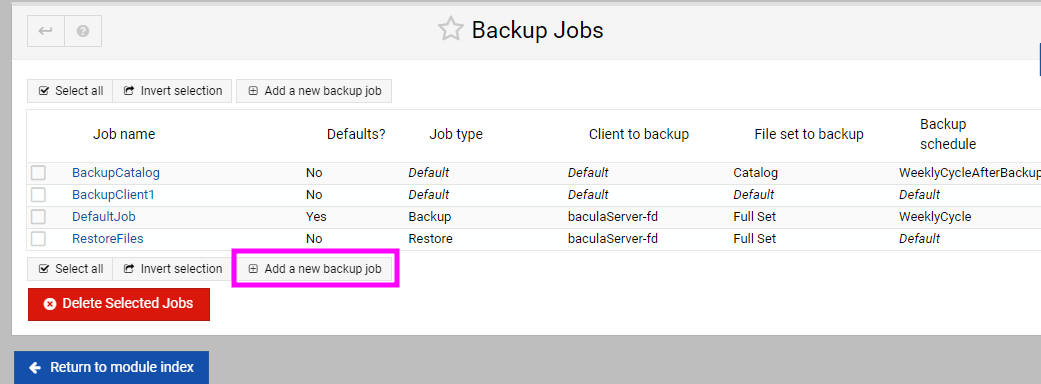
\includegraphics[width=0.5\linewidth]{instalacionBacula/createnewjob.png}
    \caption{Creación de un nuevo job de respaldo.}
\end{figure}

Los detalles para configurar el job de respaldo son:


\begin{minipage}[t]{0.45\textwidth}
    \vspace{0pt} % Alinea la parte superior de la minipágina con lo que esté al lado
    \begin{itemize}
        \item \textbf{Nombre del Job de Respaldo:} ClienteDebian1BackupJob
        \item \textbf{Tipo de Job:} Backup
        \item \textbf{Nivel de Respaldo:} Completo
        \item \textbf{Cliente a Respaldar:} baculaCliente-fd
        \item \textbf{Set de Archivos:} ClienteDebian1Archivos
        \item \textbf{Programación:} schedule1
        
    \end{itemize}

    \end{minipage}%
    \hfill % Añade espacio entre las dos minipáginas si es necesario
    \begin{minipage}[t]{0.45\textwidth}
    \vspace{0pt} % Alinea la parte superior de la minipágina con lo que esté al lado
    \centering % Centra el contenido de la minipágina
      
    

    \begin{figure}[H]
        \centering
        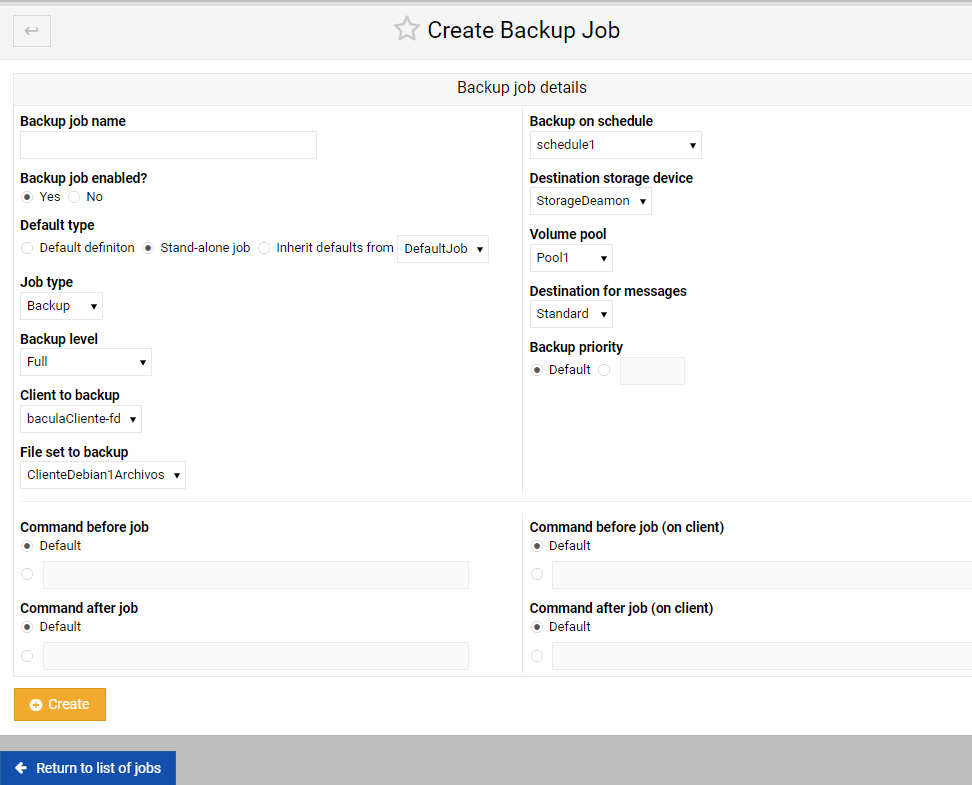
\includegraphics[width=0.95\linewidth]{instalacionBacula/Backupjobdetails.png}
        \caption{Detalles del job de respaldo configurado.}
    \end{figure}
    \end{minipage}


\smallskip

\begin{itemize}
    \item \textbf{Dispositivo de Almacenamiento Destino:} StorageDaemon
    \item \textbf{Pool de Volumen:} Pool1
    \item \textbf{Prioridad del Respaldo:} Predeterminada
\end{itemize}






\subsubsection{Ejecución de un Job de Respaldo}

Finalmente, ejecutamos el job de respaldo de manera manual para validar la configuración:

\begin{figure}[H]
    \centering
    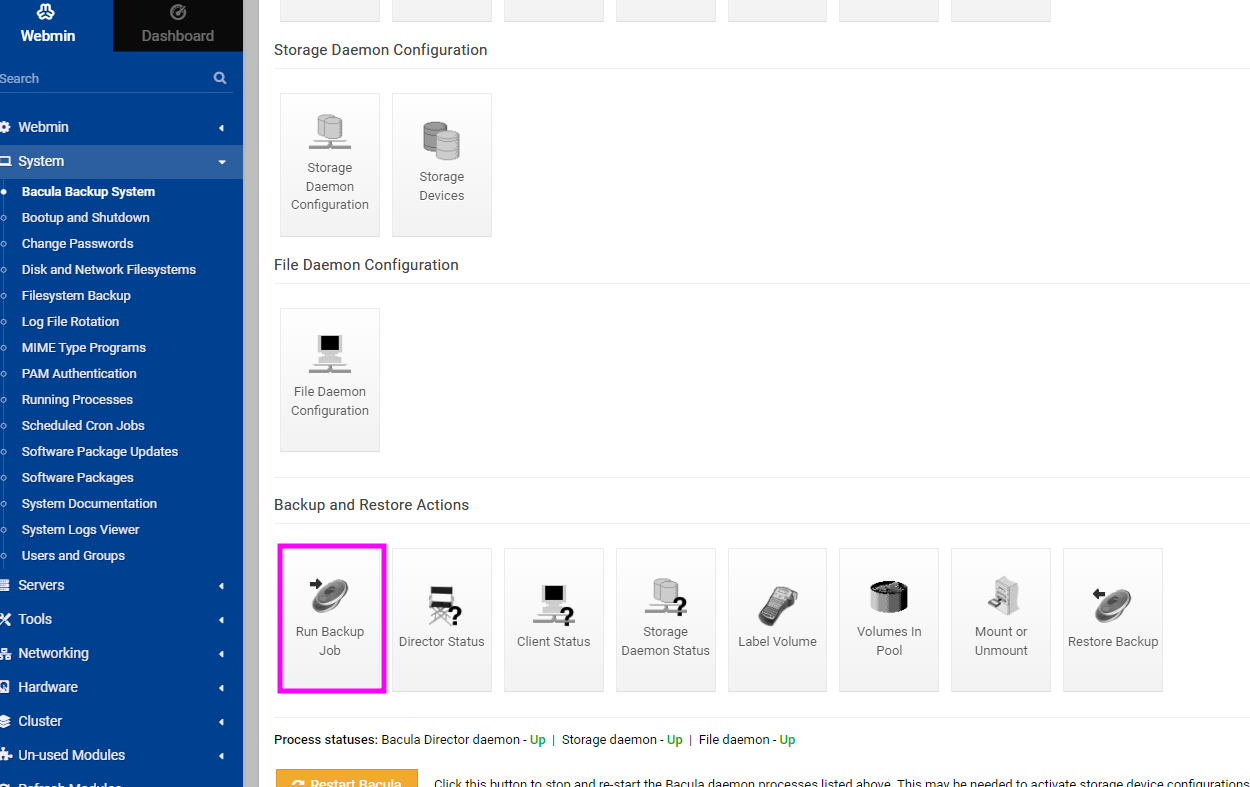
\includegraphics[width=0.5\linewidth]{instalacionBacula/runbackupjonbb.png}
    \caption{Interfaz para ejecutar un job de respaldo.}
\end{figure}

Seleccionamos el job deseado y hacemos clic en \textit{Backup Now}:

\begin{figure}[H]
    \centering
    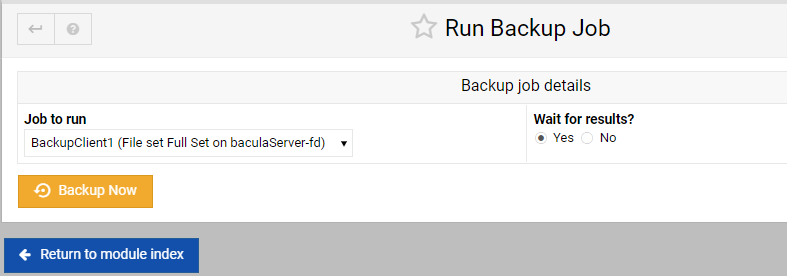
\includegraphics[width=0.5\linewidth]{instalacionBacula/backupnoww.png}
    \caption{Ejecución inmediata de un job de respaldo.}
\end{figure}

Tras la ejecución, el sistema nos proporciona un resumen detallado del proceso de respaldo:

\begin{figure}[H]
    \centering
    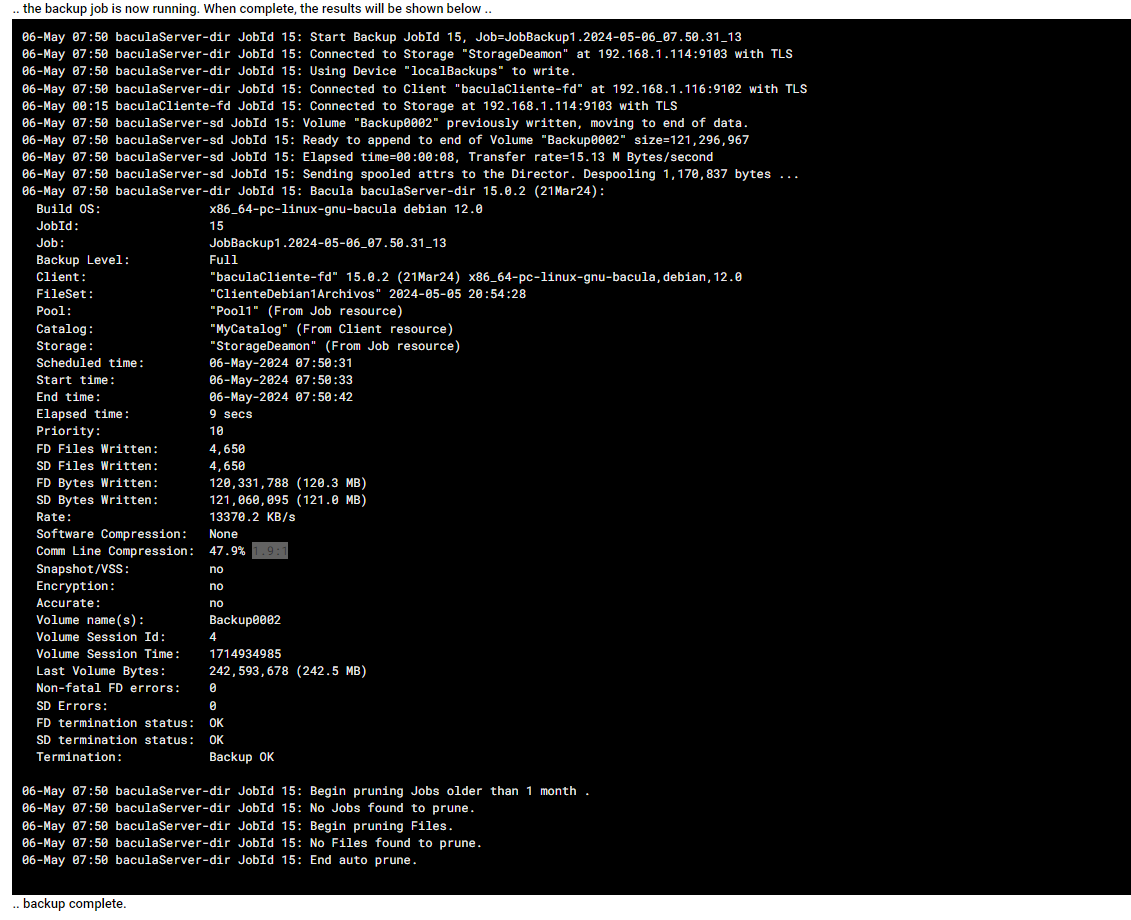
\includegraphics[width=0.5\linewidth]{instalacionBacula/salidajob1.png}
    \caption{Resultado detallado del job de respaldo ejecutado.}
\end{figure}

Con esto concluimos la configuración básica y operación del sistema de respaldos Bacula dentro de nuestra infraestructura.
